% !Mode:: "TeX:UTF-8"
% !TEX program  = xelatex
\documentclass[a4paper]{article}
\usepackage{amsmath}
\usepackage{amssymb}
\usepackage{bm}
\usepackage{ctex}
\usepackage{caption}
%\usepackage{braket}
%\usepackage[european]{circuitikz}
\usepackage{multirow}
\usepackage{float}
\usepackage{graphicx}
\usepackage{wrapfig}
\usepackage{geometry}
\geometry{left=2.5cm,right=2.5cm,bottom=2.5cm,top=2.5cm}
\title{近代物理实验报告2.4:塞曼效应}
\author{xy\quad 学号\quad 匡亚明学院}
\date{2019年2月29日}
\begin{document}
\maketitle
\bibliographystyle{unsrt}
%--------main-body------------

\section{引言}
19世纪伟大的物理学家法拉第研究电磁场对光的影响时,发现了磁场能改变偏振光的偏振方向。1896年荷兰物理学家塞曼(Pieter Zeeman)根据法拉第的想法,探测磁场对谱线的影响,发现钠双线在强磁场中的分裂。洛伦兹根据经典电子论解释了分裂为三条谱线的正常塞曼效应。由于研究这个效应,塞曼和洛伦兹共同获得了1902年的诺贝尔物理学奖。他们这一重要研究成就,有力地支持了光地电磁理论,使我们对物质地光谱、原子和分子地结构有了更多地了解。

\section{实验目的}
\begin{enumerate}
\item 掌握塞曼效应理论,测定电子的荷质比。
\item 掌握法布里—珀罗标准具的原理和使用,学习用CCD及多媒体计算机测量实验图像的方法。
\end{enumerate}

\section{实验仪器}
微机化塞曼效应实验仪。

\section{实验原理}
当光源放在足够强的磁场中时,所发出的光谱线都分裂成几条,条数随能级的类别而不同,而分裂后的谱线是偏振的,这种现象被称为塞曼效应。塞曼效应证实了原子具有磁距和空间取向量子化的现象,至今塞曼效应仍是研究能级结构地重要方法之一。

正常塞曼效应是指那些谱线分裂为三条,而且裂距(相邻两条子谱线间地波数差)正好等于一个洛伦兹单位($\frac{eB}{4\pi mc}$)的效应,可用经典理论给予很好地解释。但实际上大多数谱线的分裂多于三条,谱线的裂距是($\frac{eB}{4\pi mc}$)的简单分数倍,称反常塞曼效应,它不能用经典理论解释,只有用量子理论才能得到满意的解释。
\subsection{原子的总磁矩与总动量矩的关系}
在原子物理中我们知道,原子中的电子不但有轨道运动,而且还有自旋运动。因此,原子中的电子具有轨道角动量$P_L$和轨道磁矩$\mu_L$,以及自旋角动量$P_S$和自旋磁矩$\mu_S$。它们的关系为:
\begin{align}
\mu_L &= \frac{e}{2m}P_L & P_L &= \sqrt{L(L+1)}\hbar \notag \\
\mu_S &= \frac{2}{m}P_S & P_S &= \sqrt{S(S+1)}\hbar\label{eq1}
\end{align}
式中L,S分别表示轨道量子数和自旋量子数,e,m分别为电子的电荷和质量。

\begin{wrapfigure}{r}[0pt]{0.22\textwidth}
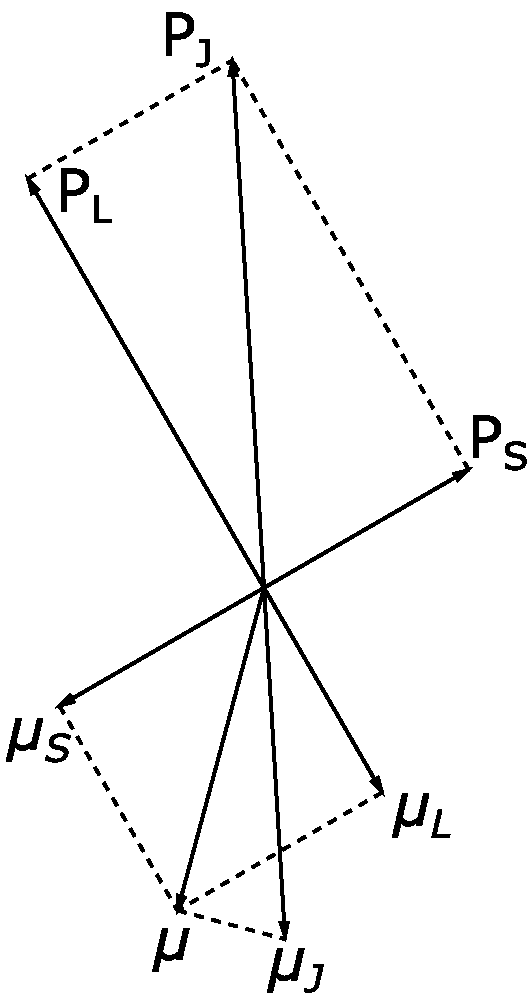
\includegraphics[width=0.22\textwidth]{fig/fig1.pdf}
\caption{电子磁矩与角动量的关系}\label{fig1}
\end{wrapfigure}

原子核也有磁矩,但它比一个电子的磁矩要小三个数量级,故在计算单电子原子的磁矩时可以把原予核的磁矩忽略,只计算电子的磁矩。

对于多电子原子,考虑到原子总角动量和总磁矩为零,故只对其原子外层价电子进行累加。磁矩的计算可用矢量图来进行,如图(\ref{fig1})。

由(\ref{eq1})式知,$\mu_S$与$P_S$的比值比$\mu_L$与$P_L$的比值大一倍,所以合成的原子总磁矩不在总动量矩$P_J$的方向上。但由于$\mu$绕$P_J$运动,只有$\mu$在$P_J$方向的投影$\mu_J$对外平均效果不为零。根据图(\ref{fig1})进行向量叠加运算,有$\mu_J$与$P_J$的关系:
\begin{equation*}
\mu_J = g\frac{e}{2m}P_J
\end{equation*}
上式中的g就是朗德因子。对于LS耦合
\begin{equation}
g = 1+\frac{J(J+1)-L(L+1)+S(S+1)}{2J(J+1)}\label{eq2}
\end{equation}
它表征了原子的总磁矩与总角动量的关系,而且决定了能级在磁场中分裂的大小。
\subsection{外磁场对原子能级作用}
原子的总磁矩在外磁场中受到力矩$\mathbf{L}$的作用。
\begin{equation}
\mathbf{L} = \bm{\mu}_J\times\mathbf{B}\label{eq3}
\end{equation}
力矩$\mathbf{L}$使总角动量发生旋进,角动量的改变的方向就是力矩的方向。原子受磁场作用而旋进所引起的附加能量$\Delta E$为:
\begin{equation}
\Delta E = -\mu_JB\cos\alpha = g\frac{e}{2m}P_J\cos\beta\label{eq4}
\end{equation}
其中角$\alpha$和$\beta$的意义如图(\ref{fig2})所示。

\begin{wrapfigure}{r}[0pt]{0.25\textwidth}
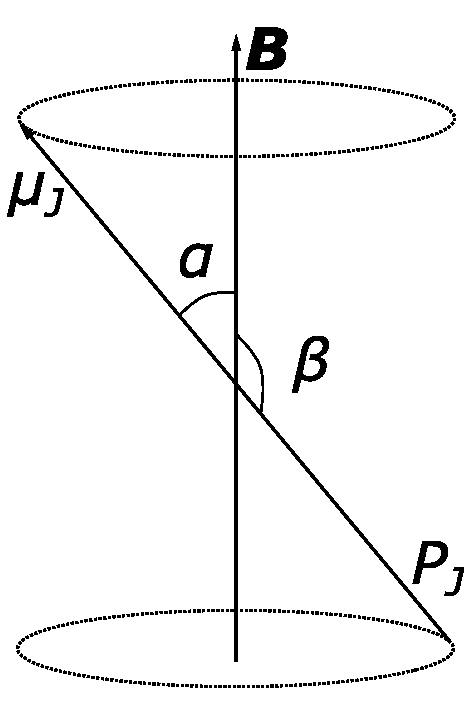
\includegraphics[width=0.25\textwidth]{fig/fig2.pdf}
\caption{原子总磁矩受磁场作用发生的旋进}\label{fig2}
\end{wrapfigure}

由于$\mu_J$或$P_J$在磁场中的取向是量子化的,也就是$P_J$在磁场方向的分量是量子化的,$P_J$的分量只能是$h$的整数倍。即
\begin{equation}
P_J\cos\beta = M\hbar\label{eq5}
\end{equation}
其中M称为磁量子数,M=J, (J-l), $\dots$ , -J,共有2J+1个M值。将(\ref{eq5})式代到(\ref{eq4})式可得
\begin{equation}
\Delta E = Mg\frac{e\hbar}{2m}B\label{eq6}
\end{equation}
这样,无外磁场时的一个能级,在外磁场的作用下可以分裂成2J+1个子能级。每个子能级的附加能量由(\ref{eq6})式决定,它正比于外磁场磁感应强度B和朗德因子g。
\subsection{塞曼效应的选择定则}
设谱线是由$E_1$和$E_2$两能级间跃迁产生的,此谱线的频率由
\begin{equation}
h\nu = E_2 - E_1\label{eq7}
\end{equation}
确定。在外场作用下的能级$E_2$和$E_1$分别分裂为(2$J_2$+l)和(2$J_l$+l)个能级,附加能量分别是$\Delta E_2$和$\Delta E_1$,产生出新的谱线频率可由
\begin{equation}
h\nu^{'} = (E_2+\Delta E_2) - (E_1+\Delta E_1)\label{eq8}
\end{equation}
确定。分裂后谱线与原谱线的频率差为:
\begin{equation}
\begin{split}
\Delta\nu &= \nu^{'} - \nu = \frac{\Delta E_2 - \Delta E_1}{h}\\
&= (M_2g_2 - M_1g_1)\frac{e}{4\pi m}\label{eq9}
\end{split}
\end{equation}
引入波数$\tilde{\nu}$,$\tilde{\nu} = \frac{\nu}{c} = \frac{1}{\lambda}$,用波数差来表示(\ref{eq9})式,有
\begin{equation}
\begin{split}
\Delta\tilde{\nu} &= (M_2g_2 - M_1g_1)\frac{e}{4\pi mc}B\\
&= (M_2g_2 - M_1g_1)L\\
&= 4.67\times 10^{-5}(M_2g_2 - M_1g_1)B(\text{cm}^{-1})\label{eq10}
\end{split}
\end{equation}
其中$L = \frac{e}{4\pi mc}$,称为洛伦兹单位,B以Gs为单位。

跃迁必须满足以下选择定则:

当M=0,垂直于磁场方向可观察到$\pi$线,为光振动方向平行于磁场方向的线偏振光(当$\Delta$J=0,$M_2$=0$\to$M=0除外。如汞的435.8nm谱线就有此情况)。平行于磁场方向观察不到$\pi$线,即其强度为零。

当M=$\pm$1,垂直于磁场方向可观察到$\sigma$线,为光振动方向垂直于磁场的线偏振光。沿磁场方向观察时,$\Delta$M=1是以磁场方向为正向的右旋偏振光,$\Delta$M=$-$1是以磁场方向为正向的左旋偏振光。对观察者而言,顺着磁场方向观察和对着磁场方向观察,偏振光方向是相反的。
\subsection{汞546.1nm谱线的塞曼分裂}
本实验的汞原子546.1nm谱线是由6s7s$^3$S$_1$跃迁到6s6p$^3$P$_2$产生的,由(\ref{eq10})式以及选择定则和偏振定则,可求出垂直于磁场观察时的塞曼分裂情况。
\begin{table}[!h]
\centering
\caption{$^3\text{S}_1$和$^3\text{P}_2$能级的各项量子数值表}\label{table1}
\begin{tabular}{|c|c|c|c|c|c|c|c|c|}
\hline
   & \multicolumn{3}{c|}{$^3\text{S}_1$} & \multicolumn{5}{c|}{$^3\text{P}_2$} \\ \hline
L  & \multicolumn{3}{c|}{0}              & \multicolumn{5}{c|}{1}              \\ \hline
S  & \multicolumn{3}{c|}{1}              & \multicolumn{5}{c|}{1}              \\ \hline
J  & \multicolumn{3}{c|}{1}              & \multicolumn{5}{c|}{2}              \\ \hline
g  & \multicolumn{3}{c|}{2}              & \multicolumn{5}{c|}{3/2}            \\ \hline
M  & 1          & 0         & -1         & 2    & 1      & 0   & -1     & -2   \\ \hline
Mg & 2          & 0         & -2         & 3    & 3/2    & 0   & -3/2   & -3   \\ \hline
\end{tabular}
\end{table}
表(\ref{table1})列出了$^3\text{S}_1$和$^3\text{P}_2$能级的各量子数L,S,J,M,g与Mg的数值。

因此,在外磁场的作用下,能级分裂情况及分裂谱线相对强度可用图(\ref{fig3})表示,图中,上面部分表示可能发生的跃迁,下面部分画出了分裂谱线的裂距与强度,将$\pi$成分画在水平线上,$\sigma$成分画在水平线下。可见汞546.1nm谱线分裂为9条等间距的谱线,相邻谱线间距都是$\frac{1}{2}$个洛伦兹单位。
\begin{figure}[!h]
\centering
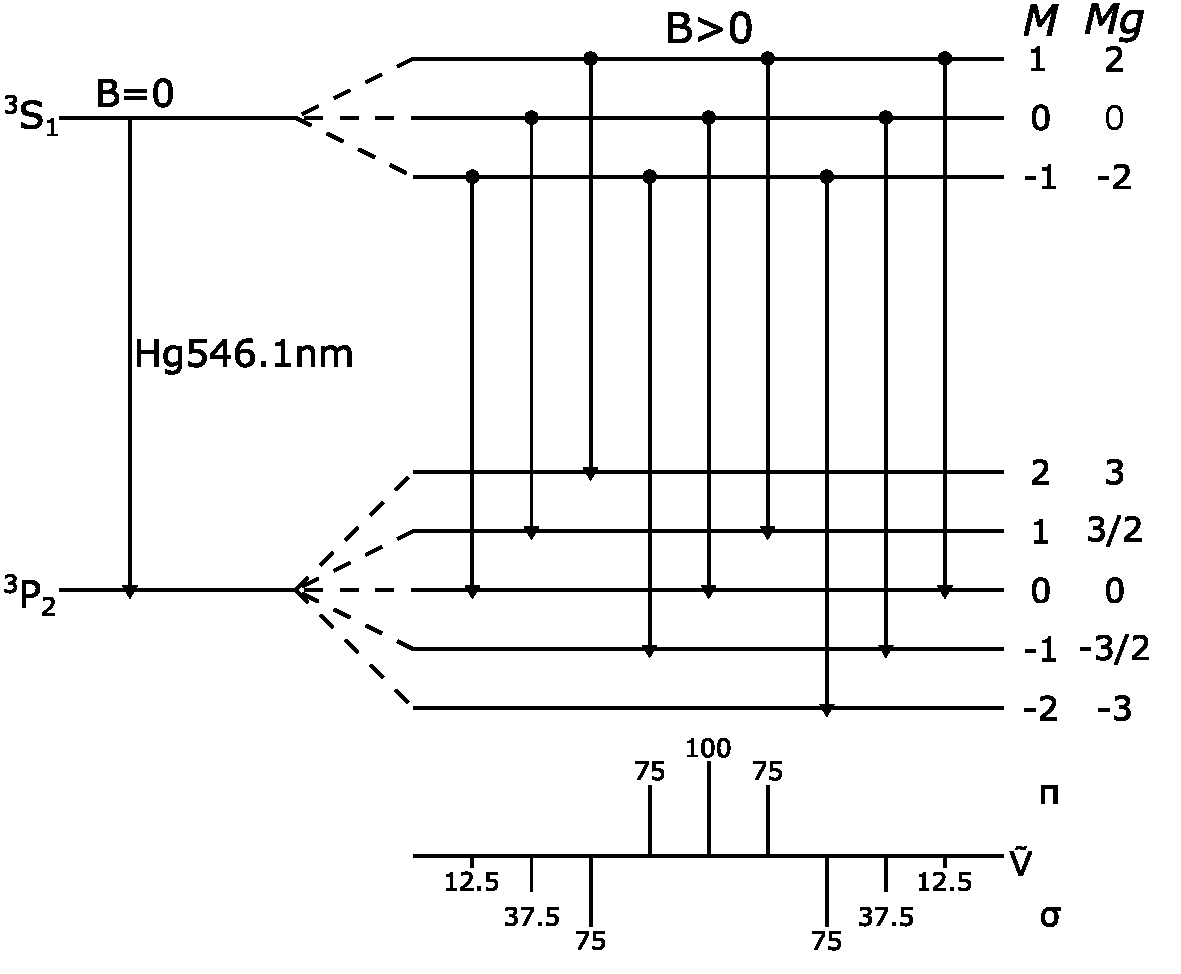
\includegraphics[width=0.8\textwidth]{fig/fig3.pdf}
\caption{能级分裂情况及谱线强度}\label{fig3}
\end{figure}

\section{实验内容}
\begin{enumerate}
\item 调整光学系统,使光束通过每个光学元件的中心(共轴调节),调节聚光透镜位置,使尽可能强的均匀光斑落在F-P的镜片上,用眼睛向F-P的出射镜片望去,可见绿光充满镜片。
\item 调节法布里-珀罗标准具。调节F-P标准具的三个压紧弹簧的螺丝,使两镜片的内表面达到严格平行,这一步骤是本实验的关键。
\item 加磁场。将汞灯置于磁铁的磁极中央,旋转偏振片的偏振方向,鉴别$\pi$成分和$\sigma$成分。
\item 选取$\pi$成分,利用CCD,通过图像卡,在计算机显示器上显示干涉圆环,并将圆环存储,再打开塞曼效应辅助分析软件,用三点决定一圆法测量干涉圆环的半径,并求出电子荷质比与实验误差,打印结果。
\end{enumerate}

\section{实验数据}

\section{误差分析}
\iffalse
\begin{enumerate}
\item 测量磁感应强度时由于磁场自身波动以及探测头的晃动,磁感应强度的数值一直在波动产生误差,并且实际的磁场不是严格的匀强磁场,磁感应强度不是处处与磁场中心(测量点)相等;
\item 测量圆环条纹的半径时,取定的三个测量点并非严格地位于同一组同心圆上,导致半径的测量存在误差。
\end{enumerate}
\fi

\section{思考题}
\subsection{对于塞曼效应的横效应,磁感应强度的最大值和最小值由什么决定?假定F-P标准具间隔圈厚度h=2mm,其最大值和最小值各是多少?}
\subsection{实验中如何鉴别成分和成分?如何观察和分辨成分中左旋和右旋圆偏振光?}

\nocite{jiaocai}
\bibliography{ref}
\end{document}